% --- Appendices ---
\appendix % Starts appendix numbering (A, B, C...)
\addcontentsline{toc}{chapter}{\appendixname}
\chapter{Приклад коду API}
\label{app:api_code_sample}

Замість простого методу створення, наведемо приклад методу для повторного надсилання листа верифікації з \texttt{AuthController}, оскільки він демонструє взаємодію з декількома сервісами та обробку специфічного сценарію користувача:
\begin{verbatim}
// Backend - AuthController - resendVerificationEmail method
@Post('resend-verification-email')
@Version('1')
@ApiOperation({ summary: 'Resend email verification link' })
@ApiBody({ schema: { properties: { email: { type: 'string', format: 'email' } } } })
async resendVerificationEmail(@Body('email') email: string) {
  return this.authService.resendVerificationEmail(email);
}

// Corresponding AuthService method snippet (conceptual)
async resendVerificationEmail(email: string): Promise<{ message: string }> {
  const user = await this.usersService.findByEmailWithDocument(email);
  if (!user) {
    throw new BadRequestException('User with this email does not exist.');
  }
  if (user.isEmailVerified) {
    throw new BadRequestException('Email is already verified.');
  }
  const verificationToken = crypto.randomBytes(32).toString('hex');
  const verificationExpires = new Date();
  verificationExpires.setHours(verificationExpires.getHours() + 1);
  await this.usersService.updateEmailVerificationToken(
    user._id.toString(), verificationToken, verificationExpires
  );
  await this.emailService.sendVerificationEmail(
    user.email, user.username, verificationToken
  );
  return { message: 'A new verification email has been sent...' };
}
\end{verbatim}

\chapter{Приклад коду клієнтської частини}
\label{app:frontend_code_sample}

Наведемо приклад функції з компонента \texttt{MapPage.tsx}, що відповідає за визначення кольору полігону поля залежно від дат обробки:
\begin{verbatim}
// Frontend - MapPage.tsx - getFieldTreatmentStatus function
const getFieldTreatmentStatus = (treatmentDates?: string[]) => {
  if (!treatmentDates || treatmentDates.length === 0) {
    return { color: 'blue', status: 'normal' }; // FIELD_COLOR_DEFAULT
  }
  const today = new Date();
  let isSoon = false;
  const TREATMENT_SOON_DAYS = 7;

  for (const dateString of treatmentDates) {
    const treatmentDate = new Date(dateString);
    // isSameDay helper function compares year, month, day
    if (isSameDay(treatmentDate, today)) {
      return { color: 'red', status: 'today' }; // FIELD_COLOR_TREATMENT_TODAY
    }
    const diffTime = treatmentDate.getTime() - today.getTime();
    const diffDays = Math.ceil(diffTime / (1000 * 60 * 60 * 24));
    if (diffDays >= 0 && diffDays <= TREATMENT_SOON_DAYS) {
      isSoon = true;
    }
  }
  if (isSoon) {
    return { color: 'orange', status: 'soon' }; // FIELD_COLOR_TREATMENT_SOON
  }
  return { color: 'blue', status: 'normal' };
};
\end{verbatim}

Також, приклад створення кастомної іконки для вуликів з використанням MUI та Leaflet:
\begin{verbatim}
// Frontend - MapPage.tsx - Custom hive icon definition
import ReactDOMServer from 'react-dom/server';
import HiveIcon from '@mui/icons-material/Hive';
import L from 'leaflet';

const hiveLeafletIcon = L.divIcon({
  html: ReactDOMServer.renderToString(<HiveIcon sx={{ fontSize: 30, color: '#FFA500' }} />),
  className: 'leaflet-mui-icon',
  iconSize: [30, 30],
  iconAnchor: [15, 30],
  popupAnchor: [0, -30]
});
// This icon is then used in <Marker icon={hiveLeafletIcon} ... />
\end{verbatim}

\chapter{Документація API (Swagger)}
\label{app:swagger_docs}
Документація API була автоматично згенерована за допомогою Swagger (OpenAPI) і доступна за ендпоінтом /docs на сервері розробки. На рисунку \ref{fig:swagger} наведено приклад головної сторінки документації, де можна переглянути доступні групи ендпоінтів (наприклад, users, forum, hives, fields) та окремі операції в межах кожної групи.

\begin{figure}[H]
  \centering
  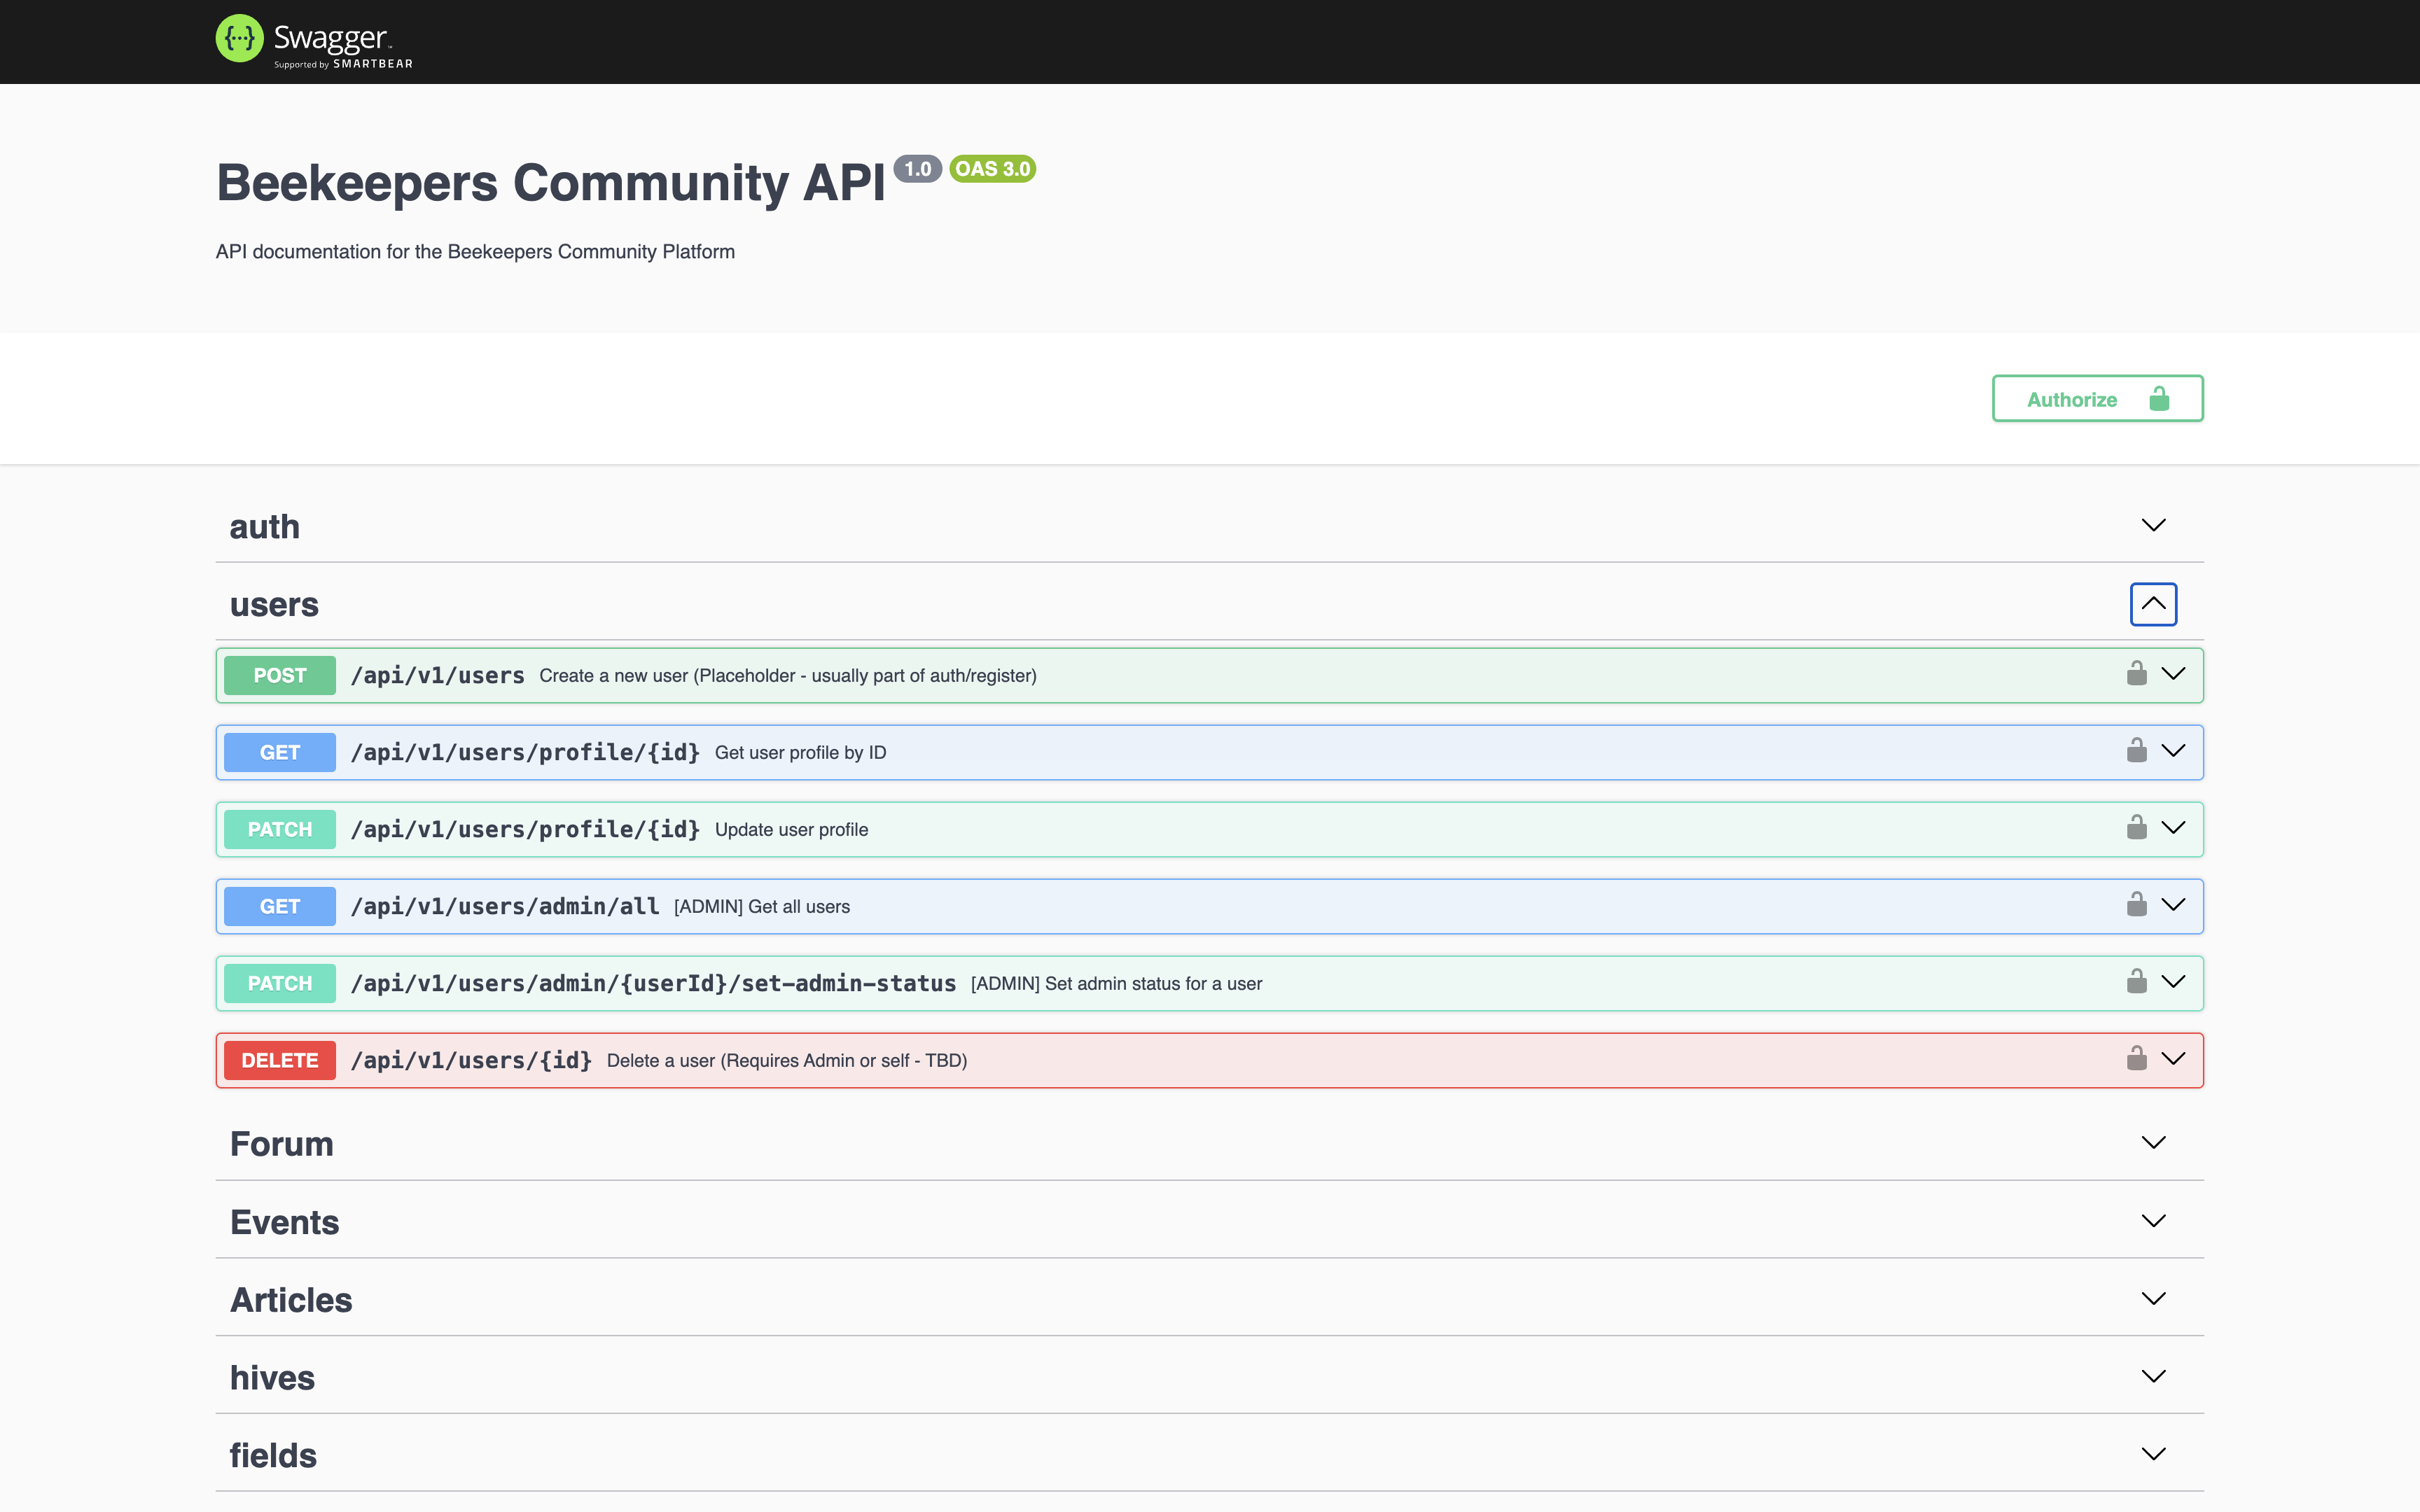
\includegraphics[width=0.9\textwidth]{practice_report/images/swagger.png}
  \caption{Головна сторінка документації API Beekeepers Community Platform у Swagger UI}
  \label{fig:swagger}
\end{figure}

\chapter{Інструкція користувача}
\label{app:user_manual}
% TODO: Provide a brief user manual for key features.

\section*{Реєстрація та вхід}
Опис процесу реєстрації та входу, включаючи верифікацію email, можливість повторного запиту листа верифікації, та вхід через Google.

\section*{Використання форуму}
Як створювати теми, писати повідомлення, коментувати.

\section*{Робота з картою}
Інтерактивна карта дозволяє користувачам управляти інформацією про свої вулики та поля.
\begin{itemize}
    \item \textbf{Додавання вулика:} Натисніть кнопку "Додати вулик", потім клікніть на карті у місці розташування вулика. У діалоговому вікні введіть назву та нотатки, потім збережіть.
    \item \textbf{Додавання поля:} Натисніть кнопку "Додати поле". Кліками на карті позначте кути вашого поля (мінімум 3 точки). Після завершення малювання натисніть "Завершити малювання". У діалоговому вікні введіть назву поля, тип культури, період цвітіння та дати запланованих обробок. Збережіть.
    \item \textbf{Перегляд інформації:} Клікніть на маркер вулика або полігон поля на карті, щоб відкрити спливаюче вікно з детальною інформацією.
    \item \textbf{Редагування поля:} У спливаючому вікні поля натисніть на іконку редагування (олівець). У діалоговому вікні, що відкриється, змініть необхідні дані та збережіть.
    \item \textbf{Видалення вулика:} У спливаючому вікні вулика натисніть на іконку видалення (кошик). Підтвердіть дію у діалоговому вікні.
    \item \textbf{Кольорове кодування полів:} Поля на карті автоматично змінюють колір для індикації статусу обробки: синій – стандартний, помаранчевий – обробка запланована протягом найближчих 7 днів, червоний – обробка запланована на сьогодні.
\end{itemize} 